Las figuras documentan lo visible en la aplicación de escritorio en el momento de la captura. La búsqueda de la Figura~\ref{fig:busqueda} muestra el término «Human» y varias coincidencias; la Figura~\ref{fig:playlist} muestra una lista propia titulada «Mi lista n.º 1», con tres canciones; y la Figura~\ref{fig:privada} muestra el control «Sesión privada» en el menú del perfil. La tercera imagen \emph{no demuestra} que una sesión privada estuviera activada ni que se ocultara efectivamente la actividad. Las capturas fueron aportadas por el estudiante; no se han simulado interfaces, ensayos ni participantes.

\begin{center}
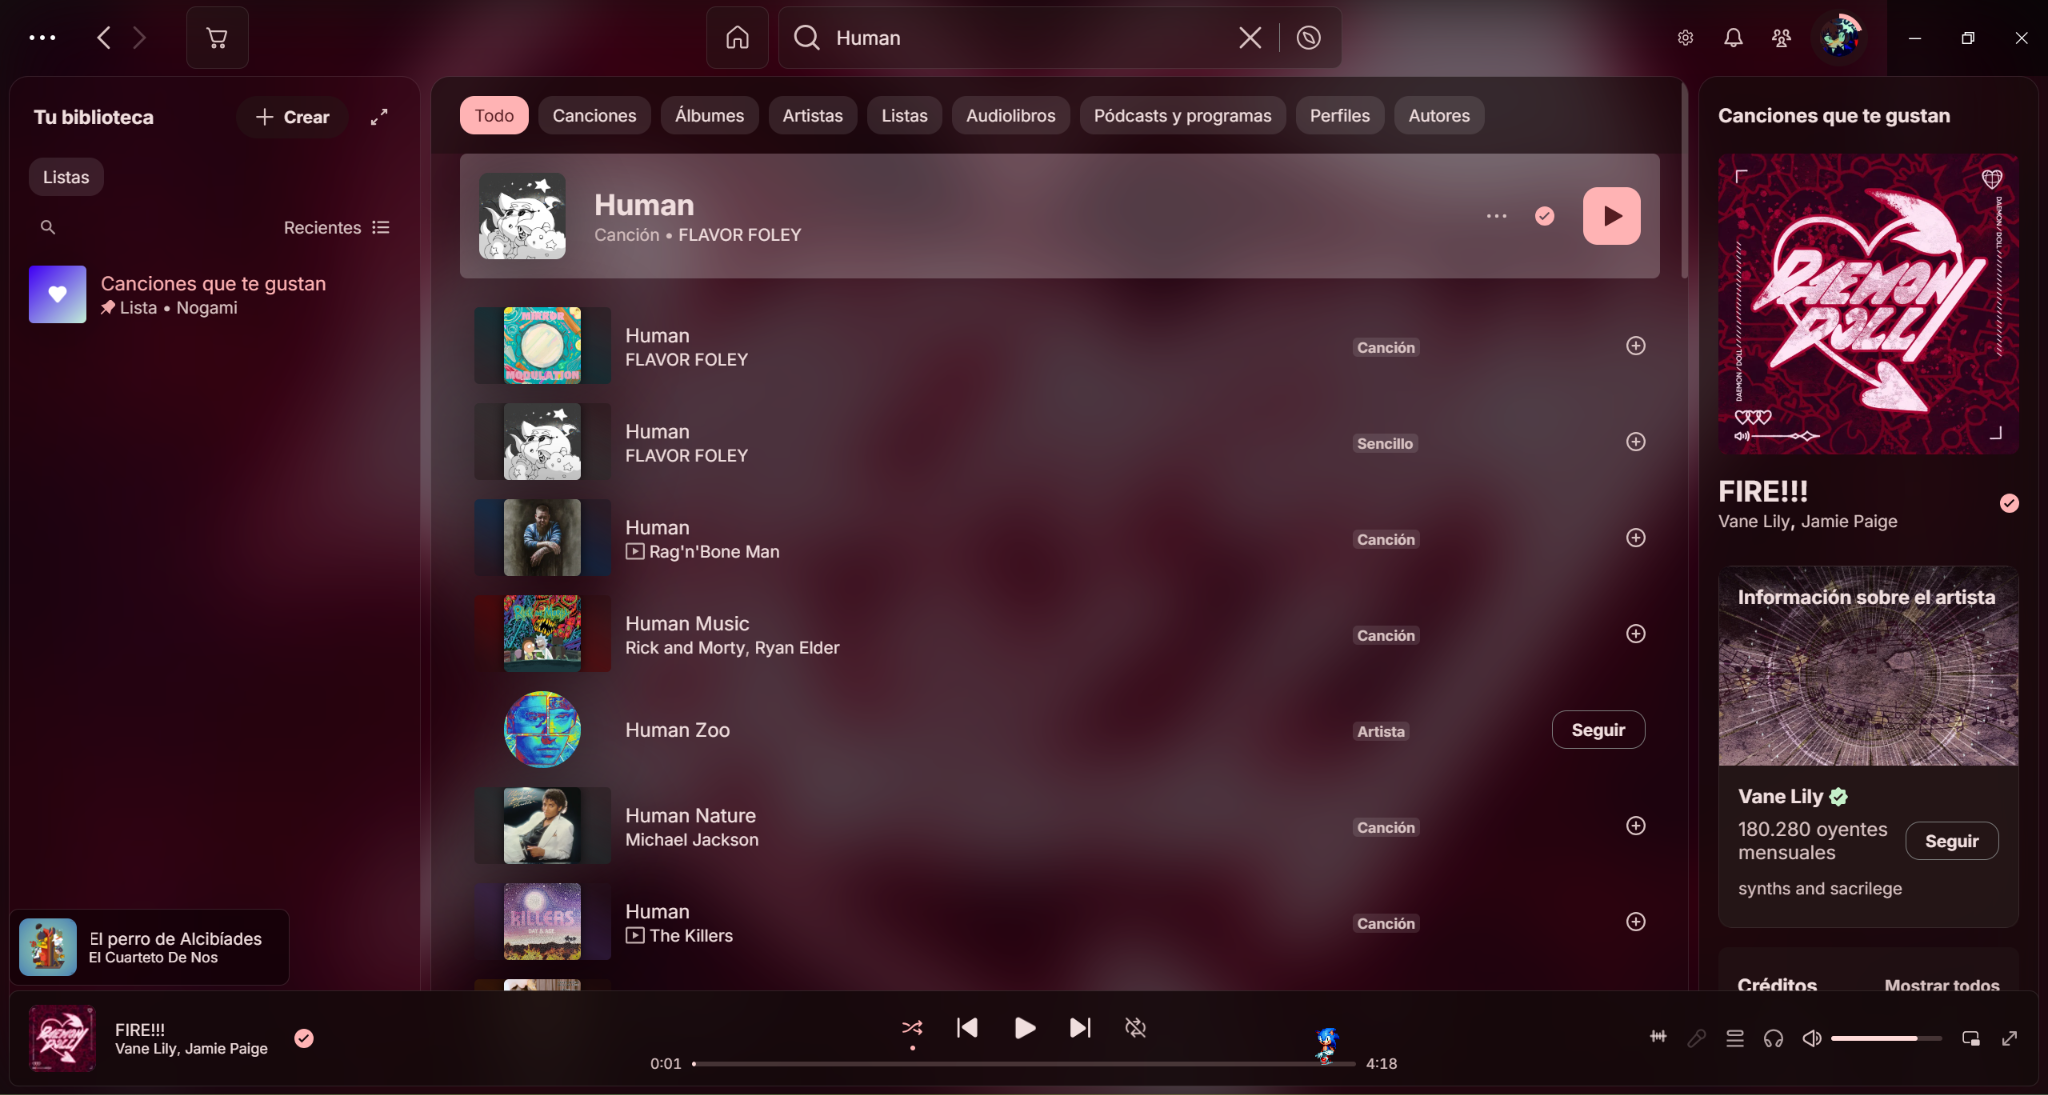
\includegraphics[width=.72\linewidth]{figuras/busqueda_spotify.png}
\captionof{figure}{Búsqueda de «Human» y resultados visibles en Spotify. Fuente: captura del estudiante.}\label{fig:busqueda}
\end{center}
\begin{center}
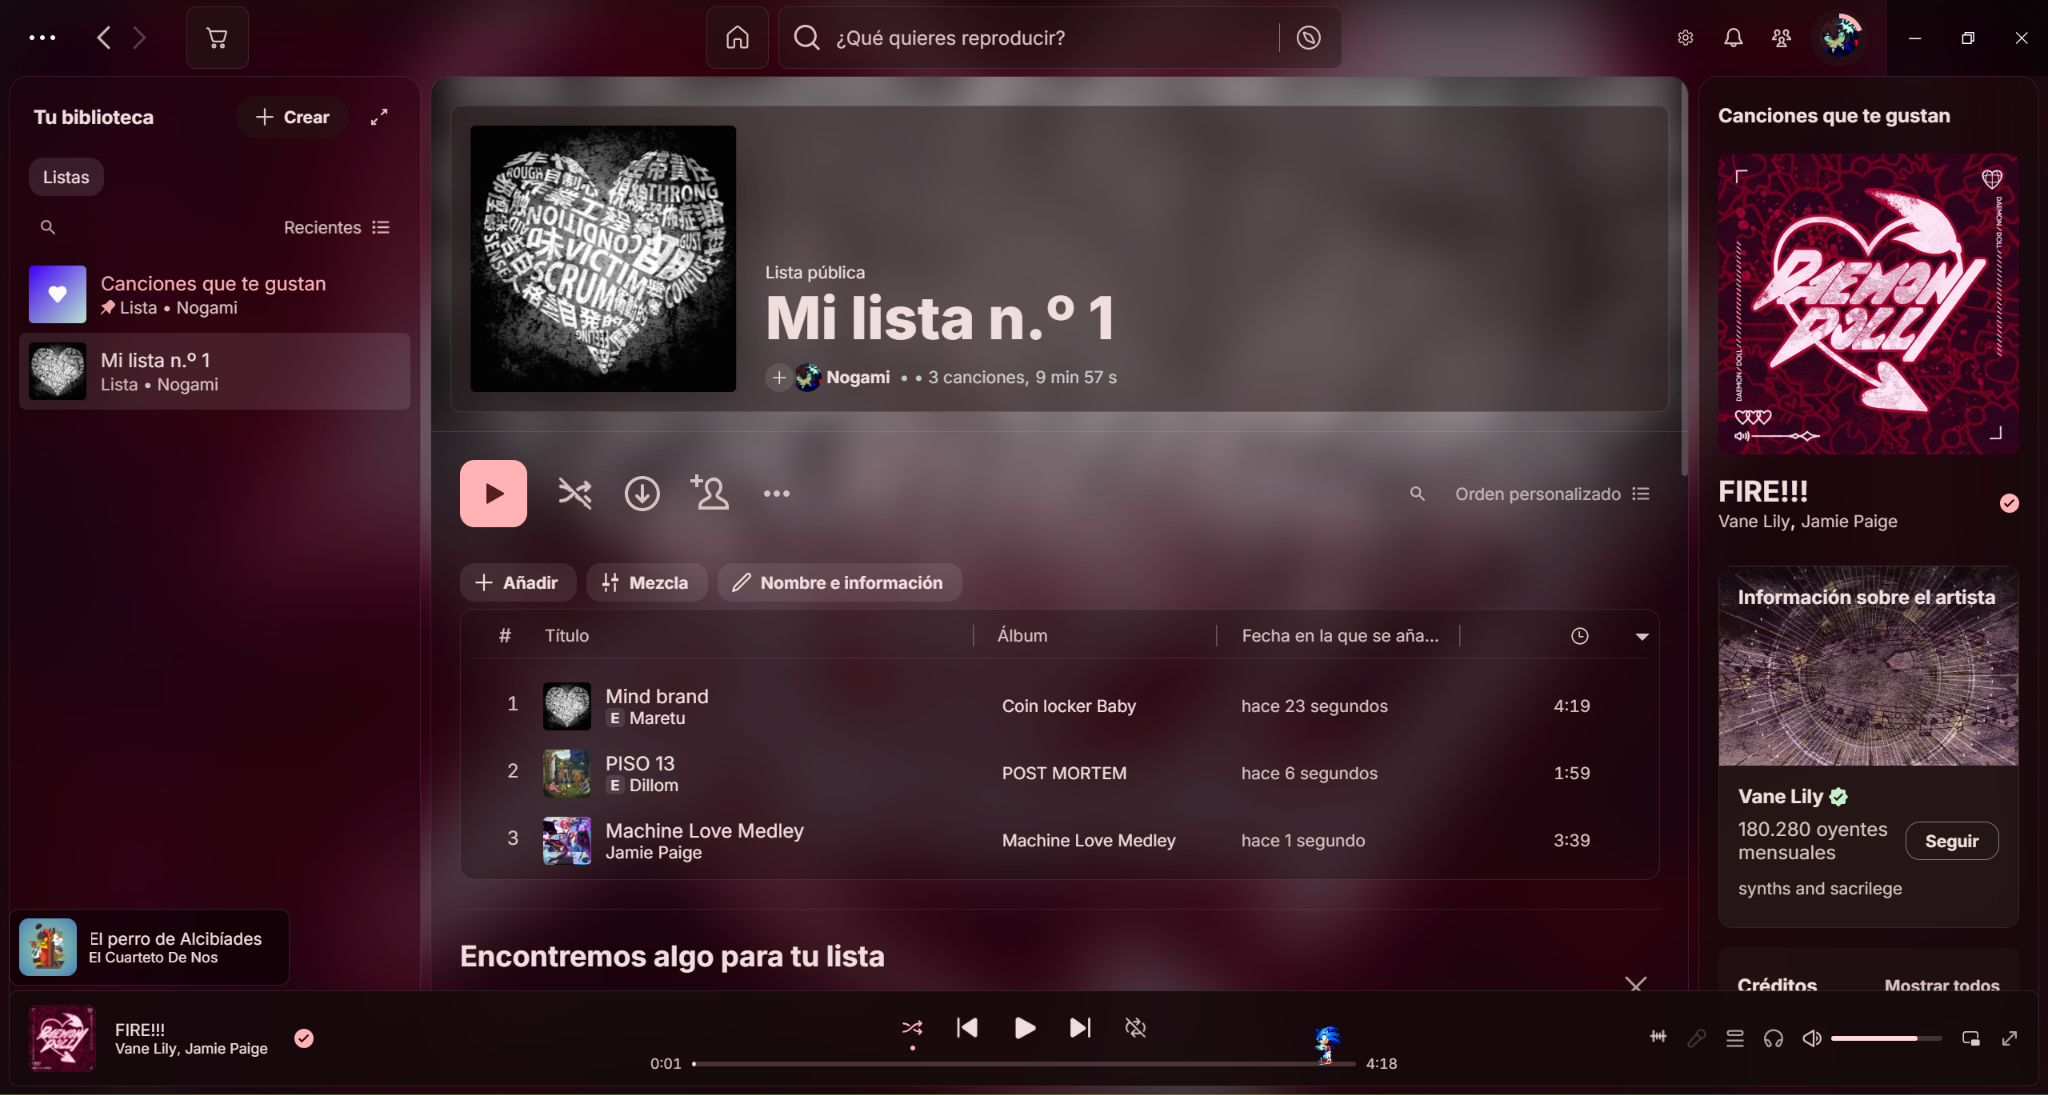
\includegraphics[width=.72\linewidth]{figuras/playlist_spotify.png}
\captionof{figure}{Lista propia con tres canciones. Fuente: captura del estudiante.}\label{fig:playlist}
\end{center}
\begin{center}
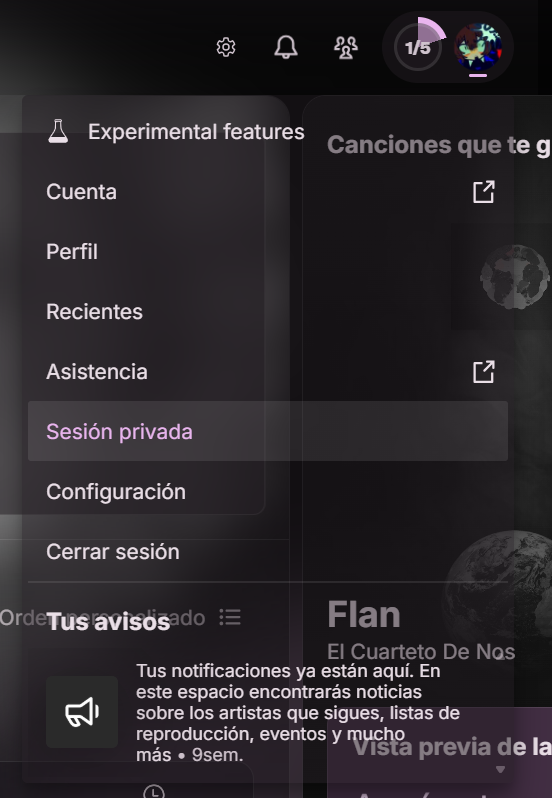
\includegraphics[height=51mm,keepaspectratio]{figuras/sesion_privada_spotify.png}
\captionof{figure}{Opción «Sesión privada» visible en el menú del perfil. Fuente: captura del estudiante.}\label{fig:privada}
\end{center}
\noindent\textbf{Alcance de la evidencia:} Figura~\ref{fig:busqueda} respalda visualmente R-04; Figura~\ref{fig:playlist} respalda la existencia del estado final de R-01 y R-02; Figura~\ref{fig:privada} respalda la disponibilidad del control relacionado con R-14, no su eficacia. Los cinco umbrales cuantitativos (R-11 a R-15) son \textbf{criterios de aceptación propuestos y pendientes de ensayo}, no resultados experimentales.
